Graphs are commonly used to describe and analyze entities with relations or interactions. Still, today's deep learning modern toolbox is specialized for simple data types, e.g., grids for images, sequences for text or speech. These data structures have spatial locality, the grid size or sequence length is fixed and can be resized. We can also determine the starting position and ending position. Graph problems are, on the other hand, much more challenging to process as they have arbitrary size and complex topological structure (i.e., no spatial locality like grids). Graphs also have no fixed node ordering or reference point compared to grids or sequences. For such Franco Scarselli et al. introduced graph neural network (GNN) \cite{graph}.

GNN is designed similarly to CNN. As previously noted, CNN operates on images. Given an image, a rectangular grid, the convolutional layer takes a subpart of the image, applies a function to it, and produces a new part, a new pixel. This is iterated for the whole image. What actually happened is the new pixel resulted in aggregated information from neighbors and itself. This cannot be easily applied to graphs as they have no spatial locality and no fixed node ordering. As implied, a GNN design stands on passing and aggregating information from neighbors. 

\subsubsection{Node embedding}

Graphs require a concept called node embedding. The general idea is to map nodes to a lower dimensional embedding space, where similar nodes in the embedding space approximate similarity in the graph network. For example, we can map a 3D vector to a 2D vector. Node embedding is useful for learning node representations and similarities and can be trained on graphs with arbitrary structures.

Nodes have embeddings at each layer. Taken node $v$, its layer-0 embedding would be its feature vector $x_v$. If we want layer-1 embedding, we will explore node $v$'s neighbors. These neighbors are so-called one hop away from our original vector $v$. We take the feature vector of these nodes and aggregate the information into one single $x_v$ feature vector. Layer-k would get information from nodes that are k hops away. 

\begin{figure}[h]
  \centering
  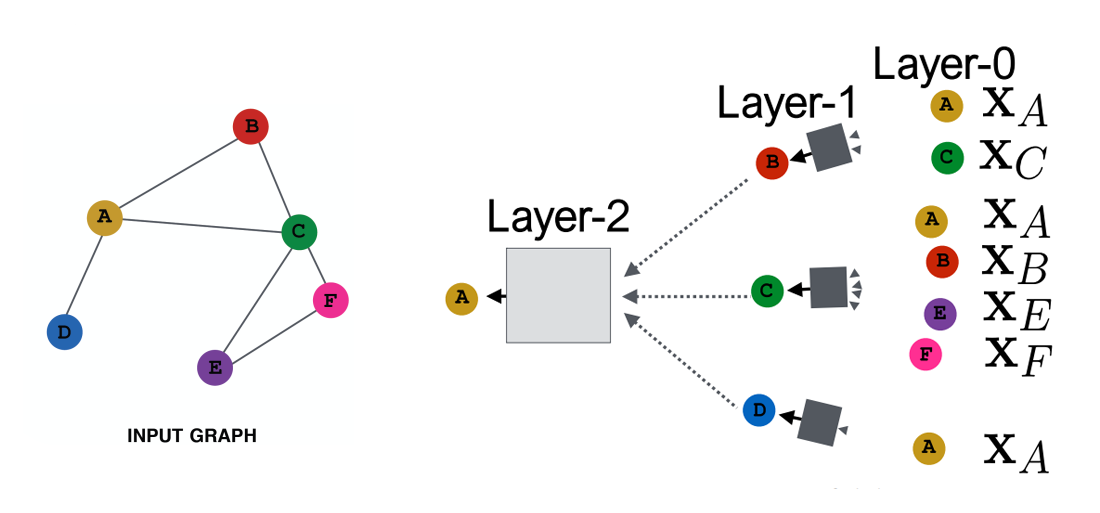
\includegraphics[width=12cm]{gnn_layers.png}
  \caption{Layer-2 embedding applied on node $A$ aggregating infromation from its neighborhood \cite{stanford}}
  \label{fig:gnn_layers}
\end{figure}

The described process is called neighborhood aggregation. If we want to predict node $v$, we need information from its neighborhood, meaning we need a way to propagate the message. Messages are passed and transformed through edges. All received messages are aggregated into a new message and then passed on. This is done systematically for every node in the graph.

The aggregation itself is done by a neural network. This implies the key difference from a typical ANN. Every node gets to define its own neural network and GNN is defined by multiple neural networks.

\begin{figure}[h]
  \centering
  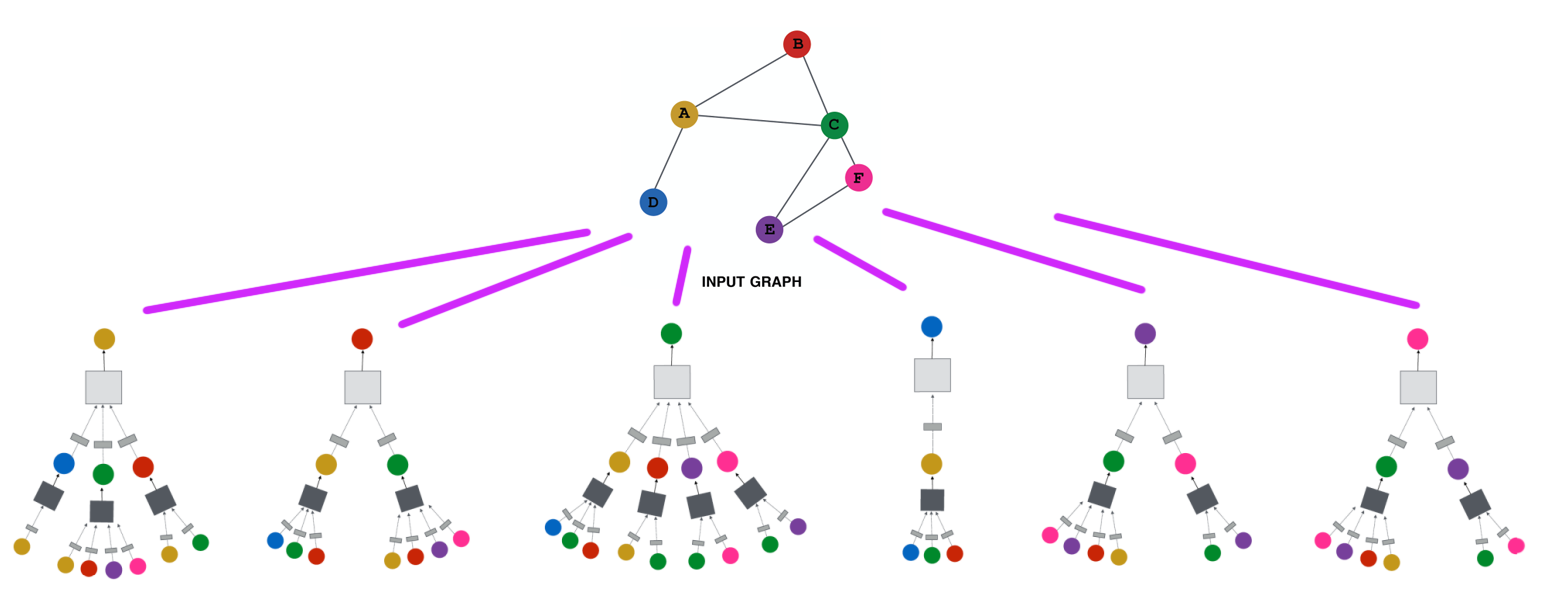
\includegraphics[width=12cm]{gnn_graph.png}
  \caption{Neural network of each node for given input node graph \cite{stanford}}
  \label{fig:gnn_graph}
\end{figure}

Using a neural network for each node in the graph, we generate a low-dimensional vector representation, embedding. The network optimizes its parameters to capture important information about the node graphs. The optimization is typically done by minimizing a loss function expressing dissimilarity between predicted and targeted node embeddings. Similar nodes are close to each other, whereas dissimilar are embedded far apart. 

\subsubsection{Geometric graphs}
TODO SECTION
Geometric graph is a graph where its nodes represent coordinates in d-dimensional space. Invariant to translation, rotation and scale

... todo more mat... 
